% Lecture Template for ME3050-001-002-Tristan Hill - Spring 2020
% Dynamics Modeling and Controls
% Second Order Time Response - Module 12 - Topic 4

% I am finally converting my stuff to BEAMER

% Document settings

%\documentclass{beamer}                  % for presentation ?
\documentclass[handout]{beamer}  % for handout ?
\usepackage{beamerthemesplit}
\usepackage{amsmath}
\usepackage{listings}
\usepackage{multicol}
\usepackage{framed}

\beamertemplateballitem

\definecolor{TTUpurple}{rgb}{0.3098, 0.1607, 0.5176} % TTU Purple (primary)
\definecolor{TTUgold}{rgb}{1.0000, 0.8666, 0.0000} % TTU Gold (primary)

\setbeamercolor{palette primary}{bg=TTUpurple,fg=TTUgold}
\setbeamercolor{palette secondary}{bg=black,fg=TTUgold}
\setbeamercolor{palette tertiary}{bg=black,fg=TTUpurple}
\setbeamercolor{palette quaternary}{bg=TTUgold,fg=black}
\setbeamercolor{structure}{fg=TTUpurple} % itemize, enumerate, etc
\setbeamercolor{section in toc}{fg=TTUpurple} % TOC sections

%\usefonttheme{professionalfonts}

\newcommand{\Lagr}{\mathcal{L}} % lagrangian

\newcommand{\hspcu}{\underline{\hspace{20mm}}} % large horizontal space w underline
\newcommand{\vspccc}{\vspace{6mm}\\} % large vertical space
\newcommand{\vspcc}{\vspace{4mm}\\}   % medium vertical space
\newcommand{\vspc}{\vspace{2mm}\\}     % small vertical space

\newcommand{\hspcccc}{\hspace{10mm}} % large horizontal space
\newcommand{\hspccc}{\hspace{6mm}} % large horizontal space
\newcommand{\hspcc}{\hspace{4mm}}   % medium horizontal space
\newcommand{\hspc}{\hspace{2mm}}     % small horizontal space

\newsavebox{\mybox} % custom box

\newcommand{\MNUM}{12\hspace{2mm}} % Module number
\newcommand{\TNUM}{4\hspace{2mm}} % Topic number 
\newcommand{\moduletitle}{Second Order Time Response} % Titles and Stuff
\newcommand{\topictitle}{Specification of The Step Response} 

\newcommand{\sectiontitleI}{The Unit Step Response} % More Titles and Stuff
\newcommand{\sectiontitleII}{Rise, Peak, and Settling Time}
\newcommand{\sectiontitleIII}{Maximum Overshoot and The Damping Ratio}
\newcommand{\sectiontitleIV}{System Identification}


\author{ME3050 - Dynamics Modeling and Controls}
\title{Module \MNUM - \moduletitle}
\date{Mechanical Engineering\vspc Tennessee Technological University}

\begin{document}

\lstset{language=MATLAB,basicstyle=\ttfamily\small,showstringspaces=false}

\frame{\titlepage \center\begin{framed}\Large \textbf{Topic \TNUM - \topictitle}\end{framed} \vspace{5mm}}

% Section 0 - Outline
\frame{
	
	\large \textbf{Topic \TNUM - \topictitle} \vspace{3mm}\\
	
	\begin{itemize}
	
		\item \sectiontitleI    \vspc % Section I
		\item \sectiontitleII 	\vspc % Section II
		\item \sectiontitleIII 	\vspc %Section III
		\item \sectiontitleIV 	\vspc %Section IV
	
	\end{itemize}

}


%Section 1: Forced Response of a Second Order Model % I think this section goes in the next lecture... 
\section{\sectiontitleI}

\frame{
\frametitle{The Mass Spring Damper}

\large Now, consider the mass-spring system with damping present subject to {\bf step} input. This models instantly turning on the input force $f(t)$.\vspc

\begin{multicols}{2}

	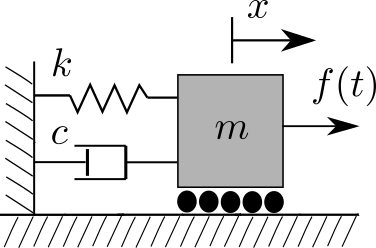
\includegraphics[scale=.4]{mass_spring_04.png} \hspc  

	\underline{Heavyside's Step Function}\vspc
	\[f(t) = \begin{cases} 
	      0 & t < 0 \\
	      F & t\geq 0 \\
	   \end{cases}
	\]\\

\end{multicols}

\large The EOM is:

	\[ m\ddot{x} +c\dot{x}+kx=f(t) \hspcc with \hspc x(t=0)=x_0 \hspcc and \hspcc v(t=0)=v_0 \] \vspc

}


\frame{ \small
\frametitle{Unit Step Response}
The {\bf unit step response} is a special case of the {\it forced response} in which $f(t)$ is the step function of unit magnitude (F=1). \vspcc
\renewcommand{\arraystretch}{2}
\begin{tabular}{|c|c|}
Overdamped & $ x(t)=\frac{1}{k}(\frac{r_2}{r_1-r_2}e^{-r_1t}-\frac{r_1}{r_1-r_2}e^{-r_2t}+1 $ \\
& $r_{1,2}=-s_{1,2}$ \\
Critically Damped & $ x(t)=\frac{1}{K}[(-1-\omega_nt)e^{-\omega_nt}+1] $ \\
Underdamped & $ x(t)=\frac{1}{k}\left[\frac{1}{\sqrt{1-\zeta^2}}e^{-\zeta\omega_nt}sin(\omega_dt+\phi+1\right] $ \\
& $ \phi=tan^{-1}\left(\frac{\sqrt{1-\zeta^2}}{\zeta}\right)+\pi $ \\
\end{tabular}

}


\frame{
\frametitle{Description and Specification of System Response}

We are going to derive several quatities that describes the response of an underdamped system. \vspc

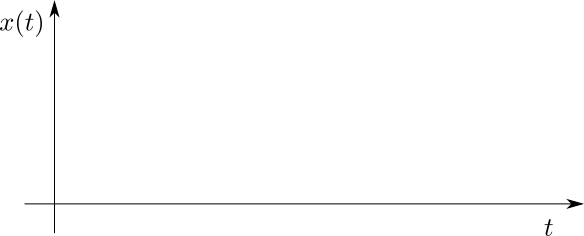
\includegraphics[scale=0.7]{lecture3_fig1.png}

}

\section{\sectiontitleII}
\frame{ \small
\frametitle{Rise Time}

The {\bf rise time} is the time at which the response first equals the steady state value.\vspc

%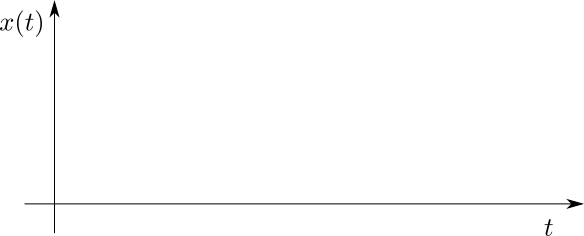
\includegraphics[scale=0.35]{lecture3_fig1.png}\vspc
\[ x(t)=\frac{1}{k}\left[\frac{1}{\sqrt{1-\zeta^2}}e^{-\zeta\omega_nt}sin(\omega_dt+\phi)+1\right] \] \vspc

Set the {\it transient term} to zero and solve for $t$.\vspc
\[ e^{-\zeta\omega_nt}sin(\omega_dt+\phi)=0 \implies sin(\omega_dt+\phi)=0\implies \omega_dt+\phi=2\pi \]
\[ t_{rise}=t_r=\frac{2\pi-\phi}{\omega_d} \]

}

\frame{ \small
\frametitle{Peak Time}

The {\bf peak time} is the time at which the response equals the maximum value. Find the derivative of the response equation and set it equal to zero. \vspc

\[ \dot{x}(t)= \]
\[ \left(\frac{1}{K}\frac{1}{\sqrt{1-\zeta^2}}\right)\left[ e^{-\zeta\omega_nt}(\omega_dcos(\omega_dt+\phi))+sin(\omega_dt+\phi)(-\zeta\omega_ne^{-\zeta\omega_nt})\right] \] \vspc
%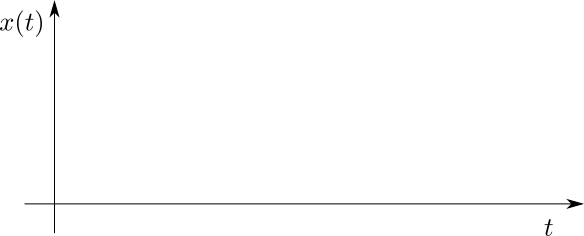
\includegraphics[scale=0.7]{lecture3_fig1.png}
\[ sin(\omega_d)t=0\implies \omega_dt=\pi \implies \hspc t_{peak}= t_p=\frac{\pi}{\omega_d} \] \vspc

}

\frame{
\frametitle{Settling Time}

The {\bf settling time} is the time at which the response decays to a certain percentage of the steady state value.\vspc

It can be esitmated as:\vspc
\[ t_{settling}=t_s=-\frac{ln(tolerance)}{\zeta\omega_n} \] \vspc
\[ 2\%\implies tolerance=0.02 \]
\[ 5\%\implies tolerance=0.05 \]
%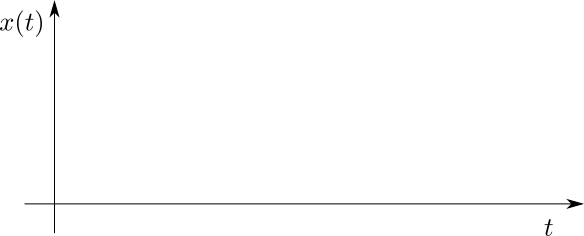
\includegraphics[scale=0.7]{lecture3_fig1.png}

}


\section{\sectiontitleIII}
\frame{
\frametitle{Maximum Overshoot}

The {\bf maximum overshoot} is the response beyond the steady state value. \vspc

\[ M_p=x(t_p)-x_{ss}\implies M_p=\frac{1}{k}e^{\frac{-\pi\zeta}{\sqrt{1-\zeta^2}}} \]\vspcc

This is often expressed as a percentage. \vspc

\[ M_\%=\frac{x(t_p)-x_{ss}}{x_{ss}}100=100e^{\frac{-\pi\zeta}{\sqrt{1-\zeta^2}} } \]

%=100e^{-\frac{\pi\zeta}{\sqrt{1-\zeta^2}}}$}
%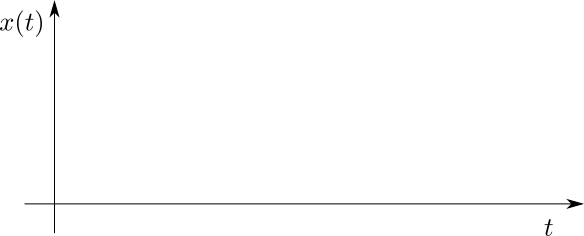
\includegraphics[scale=0.7]{lecture3_fig1.png}

}

\frame{
\frametitle{Damping Ratio from Maximum Overshoot}

The {\it damping ratio} can be determined from the maximum overshoot! \vspc

\[ M_\%=100e^{\frac{-\pi\zeta}{\sqrt{1-\zeta^2}}} \]\vspc

Solve for $\zeta$.\vspc

\[ \zeta=\frac{R}{\sqrt{\pi^2+R^2}} \hspc with \hspc R=ln\left(\frac{100}{M\%}\right) \]\vspc

}

\section{\sectiontitleIV}
\frame{ \small
\frametitle{Damping Ratio from Log Decrement}

The logarithmic decrement is the natural log of the ratio of the amplitudes of any two successive peaks: 
\[ \delta=\frac{1}{n}ln\frac{x(t)}{x(t+nT)} \]

x(t) is the overshoot (amplitude - final value) at time t and x(t + nT) is the overshoot of the peak n periods away. \vspc

The damping ratio is then found from the logarithmic decrement by: 

\[ \zeta=\frac{1}{\sqrt{1+\left(\frac{2\pi}{\delta}\right)^2}} \]

}

\frame{
\frametitle{Damping Ratio from Log Decrement}

What is the significance of all of this? \vspc
Why do we care about all of these new parameters?

}
\end{document}









 